%%%%%%%%%%%%%%%%%%%%%%%%%%%%%%%%%%%%%%%%%%%%%%%%%%%%%%%%%%%%%%%%%%%%%%
%%  Copyright by Wenliang Du.                                       %%
%%  This work is licensed under the Creative Commons                %%
%%  Attribution-NonCommercial-ShareAlike 4.0 International License. %%
%%  To view a copy of this license, visit                           %%
%%  http://creativecommons.org/licenses/by-nc-sa/4.0/.              %%
%%%%%%%%%%%%%%%%%%%%%%%%%%%%%%%%%%%%%%%%%%%%%%%%%%%%%%%%%%%%%%%%%%%%%%

\newcommand{\commonfolder}{../../common-files}
\documentclass[11pt]{article}

\usepackage[most]{tcolorbox}
\usepackage{times}
\usepackage{epsf}
\usepackage{epsfig}
\usepackage{amsmath, alltt, amssymb, xspace}
\usepackage{wrapfig}
\usepackage{fancyhdr}
\usepackage{url}
\usepackage{verbatim}
\usepackage{fancyvrb}
\usepackage{adjustbox}
\usepackage{listings}
\usepackage{color}
\usepackage{subfigure}
\usepackage{cite}
\usepackage{sidecap}
\usepackage{pifont}
\usepackage{mdframed}
\usepackage{textcomp}
\usepackage{enumitem}


% Horizontal alignment
\topmargin      -0.50in  % distance to headers
\oddsidemargin  0.0in
\evensidemargin 0.0in
\textwidth      6.5in
\textheight     8.9in 

\newcommand{\todo}[1]{
\vspace{0.1in}
\fbox{\parbox{6in}{TODO: #1}}
\vspace{0.1in}
}


\newcommand{\unix}{{\tt Unix}\xspace}
\newcommand{\linux}{{\tt Linux}\xspace}
\newcommand{\minix}{{\tt Minix}\xspace}
\newcommand{\ubuntu}{{\tt Ubuntu}\xspace}
\newcommand{\setuid}{{\tt Set-UID}\xspace}
\newcommand{\openssl} {\texttt{openssl}}


\pagestyle{fancy}
\lhead{\bfseries SEED Labs}
\chead{}
\rhead{\small \thepage}
\lfoot{}
\cfoot{}
\rfoot{}


\definecolor{dkgreen}{rgb}{0,0.6,0}
\definecolor{gray}{rgb}{0.5,0.5,0.5}
\definecolor{mauve}{rgb}{0.58,0,0.82}
\definecolor{lightgray}{gray}{0.90}


\lstset{%
  frame=none,
  language=,
  backgroundcolor=\color{lightgray},
  aboveskip=3mm,
  belowskip=3mm,
  showstringspaces=false,
%  columns=flexible,
  basicstyle={\small\ttfamily},
  numbers=none,
  numberstyle=\tiny\color{gray},
  keywordstyle=\color{blue},
  commentstyle=\color{dkgreen},
  stringstyle=\color{mauve},
  breaklines=true,
  breakatwhitespace=true,
  tabsize=3,
  columns=fullflexible,
  keepspaces=true,
  escapeinside={(*@}{@*)}
}

\newcommand{\newnote}[1]{
\vspace{0.1in}
\noindent
\fbox{\parbox{1.0\textwidth}{\textbf{Note:} #1}}
%\vspace{0.1in}
}


%% Submission
\newcommand{\seedsubmission}{You need to submit a detailed lab report, with screenshots,
to describe what you have done and what you have observed.
You also need to provide explanation
to the observations that are interesting or surprising.
Please also list the important code snippets followed by
explanation. Simply attaching code without any explanation will not
receive credits.}

%% Book
\newcommand{\seedbook}{\textit{Computer \& Internet Security: A Hands-on Approach}, 2nd
Edition, by Wenliang Du. See details at \url{https://www.handsonsecurity.net}.}

%% Videos
\newcommand{\seedisvideo}{\textit{Internet Security: A Hands-on Approach},
by Wenliang Du. See details at \url{https://www.handsonsecurity.net/video.html}.}

\newcommand{\seedcsvideo}{\textit{Computer Security: A Hands-on Approach},
by Wenliang Du. See details at \url{https://www.handsonsecurity.net/video.html}.}

%% Lab Environment
\newcommand{\seedenvironment}{This lab has been tested on our pre-built
Ubuntu 16.04 VM, which can be downloaded from the SEED website. }

\newcommand{\seedenvironmentA}{This lab has been tested on our pre-built
Ubuntu 16.04 VM, which can be downloaded from the SEED website. }

\newcommand{\seedenvironmentB}{This lab has been tested on our pre-built
Ubuntu 20.04 VM, which can be downloaded from the SEED website. }

\newcommand{\seedenvironmentAB}{This lab has been tested on our pre-built
Ubuntu 16.04 and 20.04 VMs, which can be downloaded from the SEED website. }

\newcommand{\nodependency}{Since we use containers to set up the lab environment, 
this lab does not depend too much on our SEED VM. You can do this lab
using other VMs or physical machines. }







\newcommand{\seedlabcopyright}[1]{
\vspace{0.1in}
\fbox{\parbox{6in}{\small Copyright \copyright\ {#1}\ \ by Wenliang Du.\\
      This work is licensed under a Creative Commons
      Attribution-NonCommercial-ShareAlike 4.0 International License.
      If you remix, transform, or build upon the material, 
      this copyright notice must be left intact, or reproduced in a way that is reasonable to
      the medium in which the work is being re-published.}}
\vspace{0.1in}
}






\newcommand{\telnet} {\texttt{telnet}\xspace}
\newcommand{\iptables}{\texttt{iptables}\xspace}
\newcommand{\netfilter}{\texttt{netfilter}\xspace}
\newcommand{\Netfilter}{\texttt{Netfilter}\xspace}

\newcommand{\firewallFigs}{./Figs}
\lhead{\bfseries SEED Labs -- Firewall Exploration Lab}

\newcommand{\pointleft}[1]{\reflectbox{\ding{217}} \textbf{\texttt{#1}}}

\begin{document}



\begin{center}
{\LARGE Firewall Exploration Lab}
\end{center}

\seedlabcopyright{2006 - 2021}



% *******************************************
% SECTION
% ******************************************* 
\section{Overview}

The learning objective of this lab is two-fold: learning
how firewalls work, and setting up a simple firewall
for a network. Students will first 
implement a simple stateless packet-filtering firewall, 
which inspects packets, and decides 
whether to drop or forward a packet based on firewall rules. 
Through this implementation task, students can get the 
basic ideas on how firewall works.


Actually, Linux already has a built-in firewall, also based on 
\texttt{netfilter}. This firewall is called \iptables. 
Students will be given a simple network topology, and are asked to
use \iptables to set up firewall rules to protect the network. 
Students will also be exposed to several other interesting 
applications of \iptables. 
This lab covers the following topics:


\begin{itemize}[noitemsep]
\item Firewall
\item Netfilter
\item Loadable kernel module
\item Using \iptables to set up firewall rules
\item Various applications of \iptables
\end{itemize}


\paragraph{Readings and videos.}
Detailed coverage of firewalls can be found in the following:

\begin{itemize}
\item Chapter 17 of the SEED Book, \seedbook
\item Section 9 of the SEED Lecture, \seedisvideo
\end{itemize}


\paragraph{Lab environment.} \seedenvironmentC




% *******************************************
% SECTION
% ******************************************* 
\section{Environment Setup Using Containers}


In this lab, we need to use multiple machines. 
Their setup is depicted in Figure~\ref{fig:labsetup}.  
We will use containers to set up this lab environment.


\begin{figure}[htb]
\begin{center}
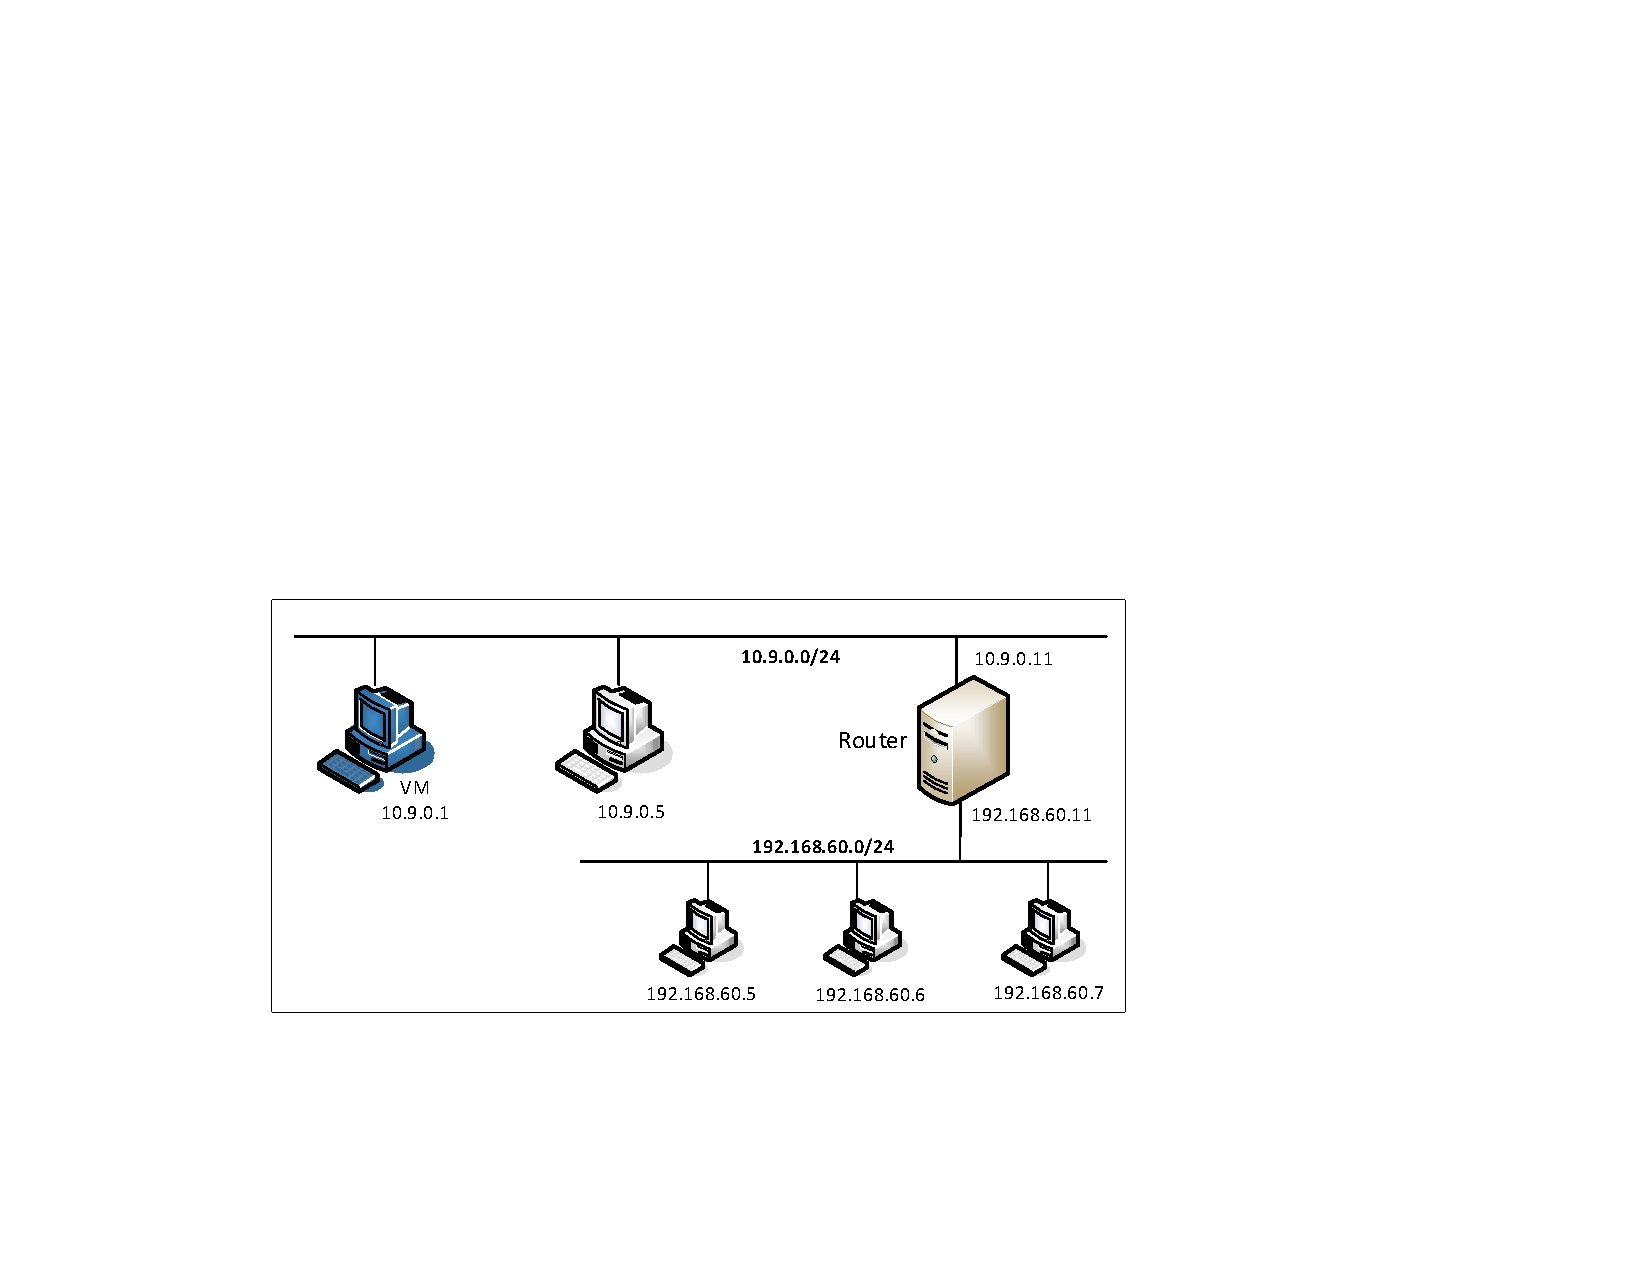
\includegraphics[width=0.8\textwidth]{./Figs/TwoLANs.pdf}
\end{center}
\caption{Lab setup}
\label{fig:labsetup}
\end{figure}


% -------------------------------------------
% SUBSECTION
% -------------------------------------------
\subsection{Container Setup and Commands}
%%%%%%%%%%%%%%%%%%%%%%%%%%%%%%%%%%%%%%%%%%%%
Please download the
\texttt{Labsetup.zip} file to your VM from the lab's website,
unzip it, enter the \texttt{Labsetup} folder, and 
use the \texttt{docker-compose.yml} file to 
set up the lab environment. Detailed explanation
of the content in this file and all the involved 
\texttt{Dockerfile} can be found from the 
user manual, which is linked to the website of this lab.
If this is the first time you set up a SEED lab environment
using containers, it is very important that you read 
the user manual. 

In the following, we list some of the commonly
used commands related to Docker and Compose. 
Since we are going to use 
these commands very frequently, we have created aliases for them
in the \texttt{.bashrc} file (in our provided SEEDUbuntu 20.04 VM).


\begin{lstlisting}
$ docker-compose build  # Build the container image
$ docker-compose up     # Start the container
$ docker-compose down   # Shut down the container

// Aliases for the Compose commands above
$ dcbuild       # Alias for: docker-compose build
$ dcup          # Alias for: docker-compose up
$ dcdown        # Alias for: docker-compose down
\end{lstlisting}


All the containers will be running in the background. To run
commands on a container, we often need to get a shell on
that container. We first need to use the \texttt{"docker ps"}  
command to find out the ID of the container, and then
use \texttt{"docker exec"} to start a shell on that 
container. We have created aliases for them in
the \texttt{.bashrc} file.

\begin{lstlisting}
$ dockps        # Alias for: docker ps --format "{{.ID}}  {{.Names}}" 
$ docksh <id>   # Alias for: docker exec -it <id> /bin/bash

# The following example shows how to get a shell inside hostC
$ dockps
b1004832e275  hostA-10.9.0.5
0af4ea7a3e2e  hostB-10.9.0.6
9652715c8e0a  hostC-10.9.0.7

$ docksh 96
root@9652715c8e0a:/#  

# Note: If a docker command requires a container ID, you do not need to 
#       type the entire ID string. Typing the first few characters will 
#       be sufficient, as long as they are unique among all the containers. 
\end{lstlisting}


If you encounter problems when setting up the lab environment, 
please read the ``Common Problems'' section of the manual
for potential solutions.


%%%%%%%%%%%%%%%%%%%%%%%%%%%%%%%%%%%%%%%%%%%%




% -------------------------------------------
% SUBSECTION
% -------------------------------------------
% It does not seem to be necessary for this lab, 
% so let's comment this out.
%\subsection{Detach the VM from \texttt{192.168.60.0/24} Network} 
%%%%%%%%%%%%%%%%%%%%%%%%%%%%%%%%%%%%%%%%%%%%
%
%\paragraph{Removing the Host VM from \texttt{192.168.60.0/24} network.}
When Docker creates a network, it automatically attach the
host machine (i.e., the VM) to the network. In this
case, the host machine is attached to both
networks, and is given the IP address \texttt{10.9.0.1} and
\texttt{192.168.60.1}.
This may create undesirable situations,
so let's remove it.

In our setup, we only want the VM to be connected to
\texttt{10.9.0.0/24}, not to both.
We need to detach the VM from the other network. We cannot simply power down
the interface, because that will affects all the containers on that network.
Our solution is to remove the IP address
of the interface, and then set the routing accordingly. 


\begin{lstlisting}
// Get the name of the interface 
$ ip addr

// Remove the IP address from the interface
$ sudo ip addr flush <interface-name>

// Use 10.9.0.11 as the router to access 192.168.60.0/24
$ sudo ip route add 192.168.60.0/24 via 10.9.0.11
\end{lstlisting}


%%%%%%%%%%%%%%%%%%%%%%%%%%%%%%%%%%%%%%%%%%%%


% *******************************************
% SECTION
% ******************************************* 
\section{Task 1: Implementing a Simple Firewall} 


In this task, we will implement a simple packet filtering 
type of firewall, which 
inspects each incoming and outgoing packets, and enforces the firewall policies 
set by the administrator. Since the packet 
processing is done within the kernel, the filtering must also be 
done within the kernel. Therefore, it seems that implementing such
a firewall requires us to modify the \linux kernel. In the past, 
this had to be done by modifying and rebuilding 
the kernel. The modern \linux 
operating systems provide several new mechanisms 
to facilitate the manipulation of packets without rebuilding
the kernel image. These two mechanisms are 
\textit{Loadable Kernel Module} (\texttt{LKM}) and \texttt{Netfilter}.



\paragraph{Notes about containers.}
Since all the containers share the same kernel, kernel modules are global. 
Therefore, if we set a kernel model from a container,
it affects all the containers and the host. For this reason, 
it does not matter where you set the kernel module. In this lab,
we will just set the kernel module from the host VM.

Another thing to keep in mind is that containers' IP addresses are virtual. 
Packets going to these virtual IP addresses may not 
traverse the same path as what is described in the Netfilter document. 
Therefore, in this task, to avoid confusion, we will try to avoid using those virtual addresses. 
We do most tasks on the host VM. The containers are mainly for the other tasks. 


% -------------------------------------------
% SUBSECTION
% ------------------------------------------- 
\subsection{Task 1.A: Implement a Simple Kernel Module}


{\tt LKM} allows us to add a new module to the kernel at the runtime. 
This new module enables us to extend the functionalities of the kernel,
without rebuilding the kernel or even rebooting the computer. 
The packet filtering part of a firewall can be implemented as an LKM. 
In this task, we will get familiar with LKM.


The following is a simple loadable kernel module. It prints out 
\texttt{"Hello World!"} when the module is loaded; when the module
is removed from the kernel, it prints out \texttt{"Bye-bye World!"}.
The messages are not printed out on the screen; they are 
actually printed into the \texttt{/var/log/syslog} file. You can
use \texttt{"dmesg"} to view the messages. 


\begin{lstlisting}[language=C, caption=\texttt{hello.c} (included in the lab setup files)]
#include <linux/module.h>
#include <linux/kernel.h>

int initialization(void)
{
    printk(KERN_INFO "Hello World!\n");
    return 0;
}

void cleanup(void)
{
    printk(KERN_INFO "Bye-bye World!.\n");
}

module_init(initialization);
module_exit(cleanup);
\end{lstlisting}

We now need to create {\tt Makefile}, which includes the following
contents (the file is included in the lab setup files). 
Just type {\tt make}, and the above program will be compiled
into a loadable kernel module (if you copy and paste the following
into \texttt{Makefile}, make sure replace the spaces before the 
\texttt{make} commands with a tab).

\begin{lstlisting}
obj-m += hello.o

all:
        make -C /lib/modules/$(shell uname -r)/build M=$(PWD) modules

clean:
        make -C /lib/modules/$(shell uname -r)/build M=$(PWD) clean
\end{lstlisting}


The generated kernel module is in \texttt{hello.ko}.  
You can use the following commands to 
load the module, list all modules, and remove the module. 
Also, you can use \texttt{"modinfo hello.ko"} to show information about a 
Linux Kernel module.

\begin{lstlisting}
$ sudo insmod hello.ko     (inserting a module)
$ lsmod | grep hello       (list modules)
$ sudo rmmod hello         (remove the module)
$ dmesg                    (check the messages)
\end{lstlisting}


\paragraph{Task.} Please compile this simple kernel module on 
your VM, and run it on the VM. For this task, we will not use 
containers.  Please show your running results in the lab report. 


% -------------------------------------------
% SUBSECTION
% ------------------------------------------- 
\subsection{Task 1.B: Implement a Simple Firewall Using \texttt{Netfilter}}  


In this task, we will write our packet filtering program
as an LKM, and then insert in into the packet processing path
inside the kernel. This cannot be easily done in the past before 
the \netfilter was introduced into the \linux.

{\tt Netfilter} is designed to facilitate the manipulation of 
packets by authorized users. It achieves this 
goal by implementing a number of hooks in the 
\linux kernel. These hooks are inserted into various places, 
including the packet incoming and outgoing paths. 
If we want to manipulate the incoming packets, we simply
need to connect our own programs (within LKM) to the 
corresponding hooks. Once an incoming packet arrives, 
our program will be invoked. Our program can decide 
whether this packet should be blocked or not; moreover,
we can also modify the packets in the program.


In this task, you need to use LKM and {\tt Netfilter} to implement
a packet filtering module.  This module will fetch 
the firewall policies from a data structure, and use the 
policies to decide whether packets should be blocked or not.
We would like students to focus on the filtering part, 
the core of firewalls, so students are allowed to hardcode firewall policies 
in the program.  Detailed guidelines on how to use \texttt{Netfilter} can be 
found in Chapter 17 of the SEED book. We will provide 
some guidelines in here as well.


\paragraph{Hooking to \texttt{Netfilter}.} 
Using \netfilter is quite straightforward. All we need to do
is to hook our functions (in the kernel module) to the corresponding
\netfilter hooks. Here we show an example (the code is in
\path{Labsetup/packet_filter}, but it may not be exactly the same as 
this example).

The structure of the code follows the structure of the kernel module 
implemented earlier. When the kernel module is added to the 
kernel, the \texttt{registerFilter()} function in the code will be 
invoked. Inside this function, we register two hooks 
to \netfilter. 

To register a hook, you need to prepare a hook data structure, 
and set all the needed parameters, the most important of which
are a function name (Line~\ding{202}) and a hook number (Line~\ding{203}). 
The hook number is one of the 
5 hooks in \netfilter, and the specified function will be 
invoked when a packet has reached this hook. In this example,
when a packet gets to the \texttt{LOCAL\_IN} hook,  the 
function \texttt{printInfo()} will be invoked (this function
will be given later). Once the hook data structure is prepared,
we attach the hook to \netfilter in Line~\ding{204}).


\begin{lstlisting}[language=C, caption={Register hook functions to \netfilter}]
static struct nf_hook_ops hook1, hook2;

int registerFilter(void) {
   printk(KERN_INFO "Registering filters.\n");
   
   // Hook 1
   hook1.hook = printInfo;                    (*@\ding{202}@*)
   hook1.hooknum = NF_INET_LOCAL_IN;          (*@\ding{203}@*)
   hook1.pf = PF_INET;
   hook1.priority = NF_IP_PRI_FIRST;
   nf_register_net_hook(&init_net, &hook1);   (*@\ding{204}@*)

   // Hook 2
   hook2.hook = blockUDP;
   hook2.hooknum = NF_INET_POST_ROUTING;
   hook2.pf = PF_INET;
   hook2.priority = NF_IP_PRI_FIRST;
   nf_register_net_hook(&init_net, &hook2);

   return 0;
}

void removeFilter(void) {
   printk(KERN_INFO "The filters are being removed.\n");
   nf_unregister_net_hook(&init_net, &hook1);
   nf_unregister_net_hook(&init_net, &hook2);
}

module_init(registerFilter);
module_exit(removeFilter);
\end{lstlisting}

\paragraph{Note for Ubuntu 20.04 VM:}
The code in the SEED book was developed in Ubuntu 16.04. It needs to be changed slightly 
to work in Ubuntu 20.04. The change is in the hook registration and 
un-registration APIs. See the difference in the following:

\begin{lstlisting}[language=C]
// Hook registration:
  nf_register_hook(&nfho);                  // For Ubuntu 16.04 VM
  nf_register_net_hook(&init_net, &nfho);   // For Ubuntu 20.04 VM

// Hook unregistration:
  nf_unregister_hook(&nfho);                // For Ubuntu 16.04 VM
  nf_unregister_net_hook(&init_net, &nfho); // For Ubuntu 20.04 VM
\end{lstlisting}
 

\paragraph{Hook functions.} We give an example of hook function
below. It only prints out the packet information.
When \netfilter invokes a hook function, it passes
three arguments to the function, including a pointer to the 
actual packet (\texttt{skb}). 
In the following code, Line~\ding{202} shows how to retrieve 
the hook number from the \texttt{state} argument. 
In Line~\ding{203}, we use \texttt{ip\_hdr()} function
to get the pointer for the IP header,
and then use the \texttt{\%pI4} format string specifier
to print out the source and destination 
IP addresses in Line~\ding{204}.

\begin{lstlisting}[language=C, caption={An example of hook function}]
unsigned int printInfo(void *priv, struct sk_buff *skb,   
                       const struct nf_hook_state *state)
{
   struct iphdr *iph;
   char *hook;

   switch (state->hook){          (*@\ding{202}@*)
     case NF_INET_LOCAL_IN: 
          printk("*** LOCAL_IN"); break;
     .. (code omitted) ...
   }

   iph = ip_hdr(skb);             (*@\ding{203}@*)           
   printk("    %pI4  --> %pI4\n", &(iph->saddr), &(iph->daddr)); (*@\ding{204}@*)
   return NF_ACCEPT;
}
\end{lstlisting}

If you need to get the headers for other protocols, you can use the following
functions defined in various header files. The  
structure definition of these headers can be found 
inside the \path{/lib/modules/5.4.0-54-generic/build/include/uapi/linux} 
folder, where the version number in the path is the result 
of \texttt{"uname -r"}, so it may be different if the kernel version
is different. 

\begin{lstlisting}[language=C]
struct iphdr   *iph   = ip_hdr(skb)    // (need to include <linux/ip.h>) 
struct tcphdr  *tcph  = tcp_hdr(skb)   // (need to include <linux/tcp.h>) 
struct udphdr  *udph  = udp_hdr(skb)   // (need to include <linux/udp.h>) 
struct icmphdr *icmph = icmp_hdr(skb)  // (need to include <linux/icmp.h>) 
\end{lstlisting}
 

\paragraph{Blocking packets.} 
We also provide a hook function example to show how 
to block a packet, if it satisfies the specified 
condition. The following example blocks the 
UDP packets if their destination IP is \texttt{8.8.8.8} 
and the destination port is \texttt{53}. This means 
blocking the DNS query to the nameserver \texttt{8.8.8.8}. 

\begin{lstlisting}[language=C, caption={Code example: blocking UDP}]
unsigned int blockUDP(void *priv, struct sk_buff *skb,
                 const struct nf_hook_state *state)
{
   struct iphdr *iph;
   struct udphdr *udph;
   u32  ip_addr;
   char ip[16] = "8.8.8.8";

   // Convert the IPv4 address from dotted decimal to a 32-bit number
   in4_pton(ip, -1, (u8 *)&ip_addr, '\0', NULL);                  (*@\ding{202}@*)
   
   iph = ip_hdr(skb);
   if (iph->protocol == IPPROTO_UDP) {
       udph = udp_hdr(skb);                                         
       if (iph->daddr == ip_addr && ntohs(udph->dest) == 53){     (*@\ding{203}@*)
            printk(KERN_DEBUG "****Dropping %pI4 (UDP), port %d\n", 
                              &(iph->daddr), port);                 
            return NF_DROP;                                       (*@\ding{204}@*)
        }
   }
   return NF_ACCEPT;                                              (*@\ding{205}@*)
}
\end{lstlisting}


In the code above, Line~\ding{202} shows, inside the kernel, 
how to convert an IP address 
in the dotted decimal format (i.e., a string, such as \texttt{1.2.3.4})
to a 32-bit binary (\texttt{0x01020304}), 
so it can be compared with the binary number stored inside packets. 
Line~\ding{203} compares the destination IP address and port 
number with the values in our specified rule. If they match the 
rule, the \texttt{NF\_DROP} will be returned to \netfilter,
which will drop the packet. Otherwise, the \texttt{NF\_ACCEPT}
will be returned, and \netfilter will let the packet 
continue its journey (\texttt{NF\_ACCEPT} only means 
that the packet is accepted by this hook function; it may still be 
dropped by other hook functions). 


\paragraph{Tasks.} The complete sample code is 
called \texttt{seedFilter.c}, which is included 
in the lab setup files (inside the \path{Files/packet_filter}
folder). Please do the following tasks (do each of them
separately):

\begin{enumerate}
\item Compile the sample code using the provided \texttt{Makefile}. 
  Load it into the kernel, and demonstrate that the firewall is working as expected. You can use
    the following command to generate UDP packets to \texttt{8.8.8.8}, which is Google's DNS
    server. If your firewall works, your request will be blocked; otherwise, you will get a
    response.

\begin{lstlisting}
dig @8.8.8.8 www.example.com 
\end{lstlisting}
     

\item Hook the \texttt{printInfo} function to all of the 
\netfilter hooks. Here are the macros of the hook numbers. 
Using your experiment results to help explain at what condition
will each of the hook function be invoked. 

\begin{lstlisting}
NF_INET_PRE_ROUTING 
NF_INET_LOCAL_IN        
NF_INET_FORWARD 
NF_INET_LOCAL_OUT 
NF_INET_POST_ROUTING    
\end{lstlisting}


\item Implement two more hooks to achieve the following:
(1) preventing other computers to ping the VM, and
(2) preventing other computers to telnet into the VM. 
Please implement two different hook functions, but register them
to the same \netfilter hook. You should decide what hook to use.
Telnet's default port is TCP port \texttt{23}. To test it, you can
start the containers, go to \texttt{10.9.0.5}, run the 
following commands (\texttt{10.9.0.1} is the IP address assigned
to the VM; for the sake of simplicity, you can hardcode this IP
address in your firewall rules):
 
\begin{lstlisting}
ping 10.9.0.1
telnet 10.9.0.1
\end{lstlisting}
     
\end{enumerate}
 

\paragraph{Important note:} Since we make changes to the kernel, there is a high chance that you would 
crash the kernel. Make sure you back up your files frequently, so you don't 
lose them. One of the common reasons for system crash is that 
you forget to unregister hooks. When a module is removed,
these hooks will still be triggered, but the module is no longer present 
in the kernel. That will cause system crash.
To avoid this, make sure for each hook you
add to your module, add a line in \texttt{removeFilter} to unregister it, 
so when the module is removed, those hooks are also removed. 


% *******************************************
% SECTION
% ******************************************* 
\section{Task 2: Experimenting with Stateless Firewall Rules}

In the previous task, we had a chance to build a simple firewall using \netfilter. Actually,
\linux already has a built-in firewall, also based on \netfilter. This firewall is called
\iptables. Technically, the kernel part implementation of the firewall
is called \texttt{Xtables}, while \iptables is a user-space program to
configure the firewall. However, \iptables is often used to refer to both the kernel-part
implementation and the user-space program. 



% -------------------------------------------
% SUBSECTION
% ------------------------------------------- 
\subsection{Background of \iptables}

In this task, we will use \iptables to set up a firewall. 
The \iptables firewall is designed not only to filter packets, but also to make changes to
packets. To help manage these firewall rules for different purposes, \iptables organizes all
rules using a hierarchical structure: table, chain, and rules.
There are several tables, each specifying the main purpose of the rules as shown
in Table~\ref{firewall:table:iptables}.
For example, rules for packet filtering should be
placed in the \texttt{filter} table, while rules for making changes to packets should be placed
in the \texttt{nat} or \texttt{mangle} tables.

Each table contains several chains, each of which corresponds to a \netfilter hook. Basically,
each chain indicates where its rules are enforced. For example, rules on
the \texttt{FORWARD} chain are enforced at the \texttt{NF\_INET\_FORWARD} hook, and rules on
the \texttt{INPUT} chain are enforced at the  \texttt{NF\_INET\_LOCAL\_IN} hook.

Each chain contains a set of firewall rules that will be enforced.
When we set up firewalls, we add rules to these chains.
For example, if we would like to block all incoming \telnet traffic, we would
add a rule to the \texttt{INPUT} chain of the \texttt{filter} table.  If we
would like to redirect all incoming \telnet traffic to a different
port on a different host, basically doing port forwarding, we can add a rule to the
\texttt{INPUT} chain of the \texttt{mangle} table, as we need to make changes to packets.


\begin{table}[htb]
        \centering
%       \renewcommand{\arraystretch}{1.2}
        \caption{\iptables Tables and Chains}
        \label{firewall:table:iptables}
        \centering

        \begin{tabular}{|l|l|l|}
                \hline
                \bfseries Table & \bfseries Chain & \bfseries Functionality \\
                \hline\hline
                filter          &    \texttt{INPUT}      & Packet filtering \\
                                &    \texttt{FORWARD}    & \\
                                &    \texttt{OUTPUT}      & \\
                \hline
                nat             &   \texttt{PREROUTING}    & Modifying source or destination \\
                                &   \texttt{INPUT}      & network addresses \\
                                &   \texttt{OUTPUT}      & \\
                                &   \texttt{POSTROUTING}   & \\
                \hline
                mangle          &   \texttt{PREROUTING}    & Packet content modification \\
                                &   \texttt{INPUT}      & \\
                                &   \texttt{FORWARD}     & \\
                                &   \texttt{OUTPUT}      & \\
                                &   \texttt{POSTROUTING}   & \\
                \hline
        \end{tabular}
\end{table}


% -------------------------------------------
% SUBSECTION
% ------------------------------------------- 
\subsection{Using \iptables}


To add rules to the chains in each table, we use the \iptables command,
which is a quite powerful command. 
Students can find the manual of \iptables by typing \texttt{"man iptables"} 
or easily find many tutorials from online. 
What makes \iptables complicated is the many command-line arguments 
that we need to provide when
using the command. However, 
if we understand the structure of these command-line arguments, 
we will find out that the command is not that complicated. 


In a typical \iptables command, we add a rule to or remove a rule 
from one of the chains in one of the tables, so we need to 
specify a table name (the default is \texttt{filter}), a chain name, 
and an operation on the chain. After that, we specify the rule, which
is basically a pattern that will be matched with each of the 
packets passing through. If there is a match, an action will be 
performed on this packet. 
The general structure of the command is depicted in the following:

\begin{lstlisting}
iptables -t <table> -<operation> <chain>  <rule>   -j <target>
         ---------- --------------------  -------  -----------
            Table          Chain           Rule      Action
\end{lstlisting}


The rule is the most complicated part of the \iptables command. 
We will provide additional information later when we use 
specific rules. In the following, we list some commonly 
used commands: 


\begin{lstlisting}
// List all the rules in a table (without line number)
iptables -t nat -L -n

// List all the rules in a table (with line number)
iptables -t filter -L -n --line-numbers


// Delete rule No. 2 in the INPUT chain of the filter table 
iptables -t filter -D INPUT 2

// Drop all the incoming packets that satisfy the <rule>
iptables -t filter -A INPUT <rule>  -j DROP
\end{lstlisting}


\paragraph{Note.} Docker relies on \iptables to manage 
the networks it creates, so it adds many rules to 
the \texttt{nat} table. 
When we manipulate \iptables rules, we should be careful 
not to remove Docker rules. For example, it will be quite
dangerous to run the \texttt{"iptables -t nat -F"} command, because 
it removes all the rules in the \texttt{nat} table,
including many of the Docker rules. That will cause 
trouble to Docker containers. Doing this for 
the \texttt{filter} table is fine, because Docker 
does not touch this table. 


% -------------------------------------------
% SUBSECTION
% -------------------------------------------
\subsection{Task 2.A: Protecting the Router} 

In this task, we will set up rules to prevent outside machines from 
accessing the router machine, except ping.   
Please execute the following \iptables
command on the router container, and then try to 
access it from \texttt{10.9.0.5}. (1) Can you ping 
the router? (2) Can you telnet into the router (a 
telnet server is running on all the containers; an
account called \texttt{seed} was created on them with
a password \texttt{dees}). 
Please report your observation and explain the purpose for 
each rule. 

\begin{lstlisting}
iptables -A INPUT  -p icmp --icmp-type echo-reply   -j ACCEPT
iptables -A OUTPUT -p icmp --icmp-type echo-request -j ACCEPT
iptables -P OUTPUT DROP     (*@\pointleft{Set default rule for OUTPUT}@*)
iptables -P INPUT  DROP     (*@\pointleft{Set default rule for INPUT}@*)
\end{lstlisting}
 

\paragraph{Cleanup.} 
Before moving on to the next task, please restore the \texttt{filter} 
table to its original state by running the following commands:

\begin{lstlisting}
iptables -F
iptables -P OUTPUT ACCEPT
iptables -P INPUT  ACCEPT
\end{lstlisting}
 
Another way to restore the states of all the tables is to restart the 
container. You can do it using the following command (you need 
to find the container's ID first):

\begin{lstlisting}
$ docker restart <Container ID>
\end{lstlisting}
 


% -------------------------------------------
% SUBSECTION
% -------------------------------------------
\subsection{Task 2.B: Protecting the Internal Network} 

In this task, we will set up firewall rules on the router to protect the 
internal network \texttt{192.168.60.0/24}. We need to use the 
FORWARD chain for this purpose. 

The directions of packets in the INPUT and OUTPUT chains are clear:
packets are either coming into (for INPUT) or going out (for OUTPUT). 
This is not true for the FORWARD chain, because it is 
bi-directional: packets going into
the internal network or going out to the external network
all go through this chain. To specify the direction,
we can add the interface options using \texttt{"-i xyz"} (coming in from 
the \texttt{xyz} interface) and/or \texttt{"-o xyz"} (going out 
from the \texttt{xyz} interface). The interfaces 
for the internal and external networks are different.
You can find out the interface names via the 
\texttt{"ip addr"} command.


In this task, we want to implement a firewall to protect the 
internal network. More specifically, we need to enforce the 
following restrictions on the ICMP traffic: 

\begin{enumerate}[noitemsep]
  \item Outside hosts cannot ping internal hosts. 
  \item Outside hosts can ping the router.
  \item Internal hosts can ping outside hosts. 
  \item All other packets between the internal and external networks should be blocked.
\end{enumerate}

You will need to use the \texttt{"-p icmp"} options to specify the match
options related to the ICMP protocol. You can run 
\texttt{"iptables -p icmp -h"} to find out all the ICMP match
options. The following example drops the ICMP echo request.


\begin{lstlisting}
iptables -A FORWARD -p icmp --icmp-type echo-request -j DROP
\end{lstlisting}

In your lab report, please include your rules and  
screenshots to demonstrate that your firewall works as expected.
When you are done with this task,
please remember to clean the table or restart the container 
before moving on to the next task.


% -------------------------------------------
% SUBSECTION
% -------------------------------------------
\subsection{Task 2.C: Protecting Internal Servers}

In this task, we want to protect the TCP servers 
inside the internal network (\texttt{192.168.60.0/24}). 
More specifically, we would like to achieve the following objectives.

\begin{enumerate}[noitemsep]
  \item All the internal hosts run a telnet server (listening to port \texttt{23}). 
    Outside hosts can only access the telnet server on \texttt{192.168.60.5},
    not the other internal hosts.

  \item Outside hosts cannot access other internal servers. 

  \item Internal hosts can access all the internal servers.

  \item Internal hosts cannot access external servers.

  \item In this task, the connection tracking mechanism is not allowed. 
    It will be used in a later task. 
\end{enumerate}

You will need to use the \texttt{"-p tcp"} options to specify the match
options related to the TCP protocol. You can run 
\texttt{"iptables -p tcp -h"} to find out all the TCP match
options. The following example allows the TCP packets coming from
the interface \texttt{eth0} if their source port is \texttt{5000}.  

\begin{lstlisting}
iptables -A FORWARD -i eth0 -p tcp --sport 5000  -j ACCEPT
\end{lstlisting}


When you are done with this task,
please remember to clean the table or restart the container 
before moving on to the next task.




% *******************************************
% SECTION
% ******************************************* 
\section{Task 3: Connection Tracking and Stateful Firewall}


In the previous task, we have only set up stateless firewalls, which inspect each
packet independently. However, packets
are usually not independent; they may be part of a TCP connection,
or they may be ICMP packets triggered by other packets. Treating them
independently does not take into consideration the context of the
packets, and can thus lead to inaccurate, unsafe, or complicated firewall rules.
For example, if we would like to allow TCP packets to get into our network
only if a connection was made first, we cannot achieve that easily 
using stateless packet filters, because when the firewall examines each individual TCP packet,
it has no idea whether the packet belongs to an existing connection
or not, unless the firewall maintains some state information for each connection.
If it does that, it becomes a stateful firewall.


% -------------------------------------------
% SUBSECTION
% ------------------------------------------- 
\subsection{Task 3.A: Experiment with the Connection Tracking} 


To support stateful firewalls, we need to be able to track connections. 
This is achieved by the \texttt{conntrack} mechanism inside the kernel. 
In this task, we will conduct experiments related to this module, and 
get familiar with the connection tracking mechanism. 
In our experiment, we will check the connection tracking information
on the router container. This can be done using the following command: 

\begin{lstlisting}
# conntrack -L
\end{lstlisting}

The goal of the task is to use a series of experiments to 
help students understand the 
connection concept in this tracking mechanism, especially
for the ICMP and UDP protocols, because unlike TCP,  they 
do not have connections. 
Please conduct the following experiments. For each experiment, please 
describe your observation, along with your explanation. 

\begin{itemize}
\item ICMP experiment: Run the following command and 
check the connection tracking information on the router. Describe
your observation. How long is the ICMP connection state be kept? 

\begin{lstlisting}
// On 10.9.0.5, send out ICMP packets
# ping 192.168.60.5
\end{lstlisting}

\item UDP experiment: Run the following command and 
check the connection tracking information on the router. Describe
your observation. How long is the UDP connection state be kept? 


\begin{lstlisting}
// On 192.168.60.5, start a netcat UDP server
# nc -lu 9090

// On 10.9.0.5, send out UDP packets  
# nc -u 192.168.60.5 9090
<type something, then hit return>
\end{lstlisting}


\item TCP experiment: Run the following command and 
check the connection tracking information on the router. Describe
your observation. How long is the TCP connection state be kept? 

\begin{lstlisting}
// On 192.168.60.5, start a netcat TCP server
# nc -l 9090

// On 10.9.0.5, send out TCP packets 
# nc 192.168.60.5 9090
<type something, then hit return>
\end{lstlisting}

\end{itemize}
 


% -------------------------------------------
% SUBSECTION
% ------------------------------------------- 
\subsection{Task 3.B: Setting Up a Stateful Firewall} 


Now we are ready to set up firewall rules based on connections. 
In the following example, 
the \texttt{"-m conntrack"} option indicates that we are using the \texttt{conntrack} module,
which is a very important module for \iptables; it tracks connections, and
\iptables replies on the tracking information to build stateful firewalls. 
The \texttt{--ctsate ESTABLISHED,RELATED} indicates that whether a packet
belongs to an \texttt{ESTABLISHED} or \texttt{RELATED} connection.
The rule allows TCP packets belonging to an existing connection to 
pass through. 

\begin{lstlisting}
iptables -A FORWARD -p tcp -m conntrack          \
         --ctstate ESTABLISHED,RELATED -j ACCEPT
\end{lstlisting}


The rule above does not cover the SYN packets, which do not belong to 
any established connection. Without it, we will not be able to 
create a connection in the first place. Therefore, we need to 
add a rule to accept incoming SYN packet: 

\begin{lstlisting}
iptables -A FORWARD -p tcp -i eth0 --dport 8080 --syn  \
         -m conntrack --ctstate NEW -j ACCEPT 
\end{lstlisting}

Finally, we will set the default policy on FORWARD to drop
everything. This way, if a packet is not accepted by the two
rules above, they will be dropped. 

\begin{lstlisting}
iptables -P FORWARD DROP
\end{lstlisting}


Please rewrite the firewall rules in Task 2.C, but this time,
\textbf{we will add a rule allowing internal hosts to visit any 
external server} (this was not allowed in Task 2.C). 
After you write the rules using the connection tracking mechanism, 
think about how to do it without using the connection tracking
mechanism (you do not need to actually implement them). 
Based on these two sets of rules, 
compare these two different approaches, and 
explain the advantage and disadvantage of each approach. 
When you are done with this task, remember to clear all the rules. 



% *******************************************
% SECTION
% ******************************************* 
\section{Task 4: Limiting Network Traffic}

In addition to blocking packets, we can also 
limit the number of packets that can pass through the firewall. 
This can be done using the \texttt{limit} module of \iptables.
In this task, we will use this module to limit how many packets 
from \texttt{10.9.0.5} are allowed to get into the internal network. 
You can use \texttt{"iptables -m limit -h"} to see the manual.  

\begin{lstlisting}
$ iptables -m limit -h
limit match options:
--limit avg             max average match rate: default 3/hour
                        [Packets per second unless followed by
                        /sec /minute /hour /day postfixes]
--limit-burst number    number to match in a burst, default 5
\end{lstlisting}
 

Please run the following commands on router, and then
ping \texttt{192.168.60.5} from \texttt{10.9.0.5}.  
Describe your observation. 
Please conduct the experiment with and without the second rule, 
and then explain whether the second rule is needed or not, and why.

\begin{lstlisting}
iptables -A FORWARD -s 10.9.0.5 -m limit \
         --limit 10/minute --limit-burst 5 -j ACCEPT

iptables -A FORWARD -s 10.9.0.5 -j DROP
\end{lstlisting}



% *******************************************
% SECTION
% *******************************************
\section{Task 5: Load Balancing}

The \iptables is very powerful. In addition to firewalls,
it has many other applications. We will not be able to 
cover all its applications in this lab, but we will experimenting
with one of the applications, load balancing. In this task,
we will use it to load balance three UDP servers running in the 
internal network. Let's first start the server
on each of the hosts: \texttt{192.168.60.5}, \texttt{192.168.60.6}, and 
\texttt{192.168.60.7} (the \texttt{-k} option indicates that 
the server can receive UDP datagrams from multiple hosts):

\begin{lstlisting}
nc -luk 8080
\end{lstlisting}

We can use the \texttt{statistic} module to achieve load balancing. 
You can type the following command to get its manual. You can 
see there are two modes: \texttt{random} and \texttt{nth}. 
We will conduct experiments using both of them.

\begin{lstlisting}
$ iptables -m statistic -h 
statistic match options:
 --mode mode         Match mode (random, nth)
 random mode:
[!] --probability p  Probability
 nth mode:
[!] --every n        Match every nth packet
 --packet p          Initial counter value (0 <= p <= n-1, default 0)
\end{lstlisting}
 

\paragraph{Using the \texttt{nth} mode (round-robin).}
On the router container, we set the following rule, which applies 
to all the UDP packets going to port \texttt{8080}. 
The \texttt{nth} mode of the \texttt{statistic} module is used; 
it implements a round-robin load balancing policy: for every
three packets, pick the packet 0 (i.e., the first one), 
change its destination IP address and port number to 
\texttt{192.168.60.5}  and \texttt{8080}, respectively.  
The modified packets will continue on its journey.

\begin{lstlisting}
iptables -t nat -A PREROUTING -p udp --dport 8080      \
         -m statistic --mode nth --every 3 --packet 0  \
         -j DNAT --to-destination 192.168.60.5:8080
\end{lstlisting}

It should be noted that those packets that do not match
the rule will continue on their journeys; they will
not be modified or blocked. With this rule in place, 
if you send a UDP packet to the router's \texttt{8080} port,  
you will see that one out of three packets gets to 
\texttt{192.168.60.5}. 

\begin{lstlisting}
// On 10.9.0.5
echo hello | nc -u 10.9.0.11 8080
<hit Ctrl-C>
\end{lstlisting}
 

Please add more rules to the router container, 
so all the three internal hosts get the equal 
number of packets. 
Please provide some explanation for the rules. 


\paragraph{Using the \texttt{random} mode.}
Let's use a different mode to achieve the load balancing. The following 
rule will select a matching packet with the probability \texttt{P}.  
You need to replace \texttt{P} with a probability number.

\begin{lstlisting}
iptables -t nat -A PREROUTING -p udp --dport 8080   \
         -m statistic --mode random --probability P \
         -j DNAT --to-destination 192.168.60.5:8080
\end{lstlisting}

Please use this mode to implement your load balancing 
rules, so each internal server get roughly the 
same amount of traffic (it may not be exactly the same, 
but should be close when the total number of packets is large). 
Please provide some explanation for the rules. 




% *******************************************
% SECTION
% ******************************************* 
\section{Submission and Demonstration}


%%%%%%%%%%%%%%%%%%%%%%%%%%%%%%%%%%%%%%%%

You need to submit a detailed lab report, with screenshots,
to describe what you have done and what you have observed.
You also need to provide explanation
to the observations that are interesting or surprising.
Please also list the important code snippets followed by
explanation. Simply attaching code without any explanation will not
receive credits.

%%%%%%%%%%%%%%%%%%%%%%%%%%%%%%%%%%%%%%%%


\end{document}
%%%%%%%%%%%%%%%%%%%%%%%%%%%%%%%%%%%%%%%%%%%%%%%%%%%%%%%%
%%%%%%%%%%%%%%%%%%%%%%%%%%%%%%%%%%%%%%%%%%%%%%%%%%%%%%%%



